\section{PlanesQML}

The last of the 3 Qt based GUIs is PlanesQML. This uses QML, a declarative language similar to html to create the graphical interfaces.

\subsection{Main Window}

The main.cpp for the project looks as follows:

\begin{lstlisting}
	QGuiApplication app(argc, argv);
	QQmlApplicationEngine engine;
	
	PlaneGameQML planeGame;
	PlaneGridQML player_pgq(&planeGame, planeGame.playerGrid());
	PlaneGridQML computer_pgq(&planeGame, planeGame.computerGrid());
	player_pgq.initGrid();
	computer_pgq.initGrid();
	
	engine.rootContext()->setContextProperty("PlayerPlaneGrid", &player_pgq);
	engine.rootContext()->setContextProperty("ComputerPlaneGrid", &computer_pgq);
	engine.rootContext()->setContextProperty("PlaneGame", &planeGame);
	engine.load(QUrl(QStringLiteral("qrc:/main.qml")));
\end{lstlisting}

The QML interpreting engine is define by an object of the type QQmlApplicationEngine. Our application implements everything in QML except for the game engine, which is implemented in C++. In order to be able to reference the C++ objects in QML, two wrapper classes were created: PlaneGameQML and PlaneGridQML. 

Here below is the header file for PlaneGameQML:

\begin{lstlisting}

class PlaneGameQML : public QObject
{
	Q_OBJECT
public:
	PlaneGameQML();
	~PlaneGameQML();

public:
	Q_INVOKABLE void doneEditing();
	Q_INVOKABLE inline int getPlayerMoves() { return m_Stats.m_playerMoves; }
	Q_INVOKABLE inline int getPlayerHits() { return m_Stats.m_playerHits; }
	Q_INVOKABLE inline int getPlayerDead() { return m_Stats.m_playerDead; }
	Q_INVOKABLE inline int getPlayerMisses() { return m_Stats.m_playerMisses; }
	Q_INVOKABLE inline int getPlayerWins() { return m_Stats.m_playerWins; }
	Q_INVOKABLE inline int getComputerMoves() { return m_Stats.m_computerMoves; }
	Q_INVOKABLE inline int getComputerHits() { return m_Stats.m_computerHits; }
	Q_INVOKABLE inline int getComputerDead() { return m_Stats.m_computerDead; }
	Q_INVOKABLE inline int getComputerMisses() { return m_Stats.m_computerMisses; }
	Q_INVOKABLE inline int getComputerWins() { return m_Stats.m_computerWins; }
	
	Q_INVOKABLE void startNewGame();
	
	inline PlaneGrid* playerGrid() { return mRound->playerGrid(); }
	inline PlaneGrid* computerGrid() { return mRound->computerGrid(); }

signals:
	void guessMade(const GuessPoint& gp);
	void computerMoveGenerated(const GuessPoint& gp);    
	void updateStats();
	void roundEnds(bool isPlayerWinner);
	void resetGrid();

public slots:
	void statsUpdated(const GameStatistics& stats);
	void receivedPlayerGuess(const GuessPoint& gp);

private:
	//The controller object
	PlaneRound* mRound;
	GameStatistics m_Stats;
};

\end{lstlisting}

Observe that the class derives from QObject and that some methodes are declared using the Qt macro Q\_INVOKABLE. This allows the methods to be accessible from the QML code. PlaneGridQML has a header file with the same characteristics.

In order to register the C++ object with the QML engine one uses the setContextProperty() function as shown above.

By using the function load() one can define the start qml object for the project: main.qml

\begin{lstlisting}

Window {
	visible: true
	width: 1000
	height: 700

Row {
	anchors.fill: parent
	LeftPane {
		id: leftPane
	}
	RightPane {
		id: rightPane
	}
	}
}
\end{lstlisting}

This defines a window with 100 X 700 size composed of two subobjects: LeftPane and RightPane, which play similar roles as in PlanesGraphicsScene.

\begin{figure}[h]
	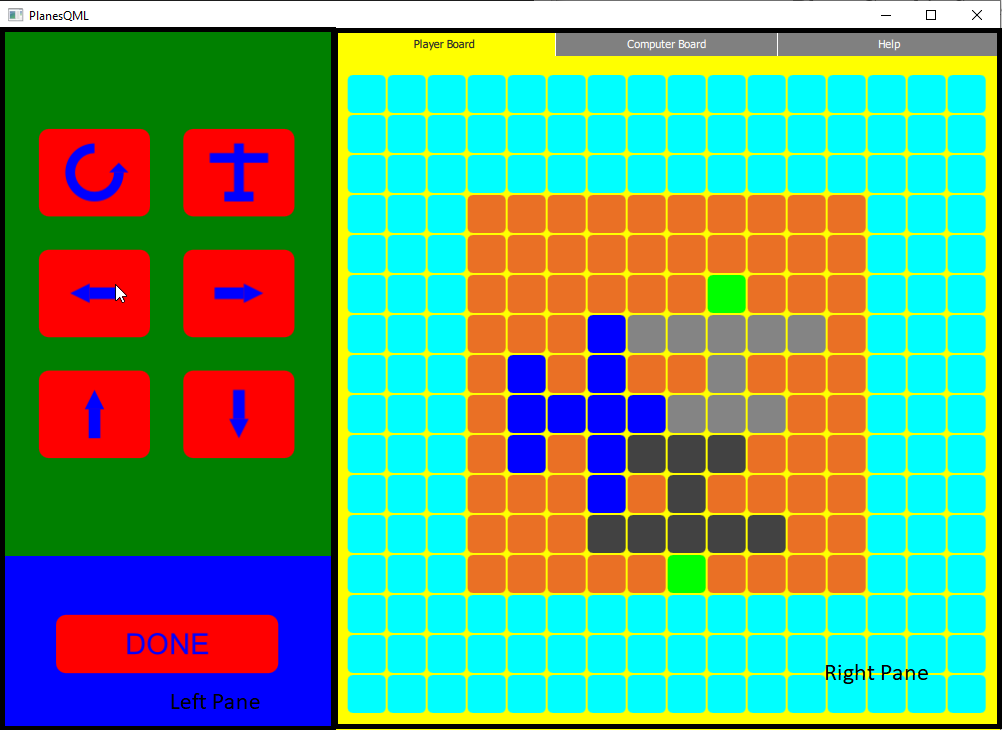
\includegraphics[width = \textwidth]{PlanesQML_BoardEditing_WidgetNames.png}
	\caption{Simplified Layout of PlanesQML}
	\label{fig:planesqml_boardediting_widgetnames}
\end{figure}

\subsection {LeftPane}


